\documentclass[calculator,steamtables]{exam}
% The full list of class options are
% calculator : Allows approved calculator use.
% datasheet : Adds a note that data sheet are attached to the exam.
% handbook : Allows the use of the engineering handbook.
% resit : Adds the resit markings to the paper.
% sample : Adds conspicuous SAMPLE markings to the paper
% solutions : Uses the contents of \solution commands (and \solmarks) to generate a solution file

\coursecode{EG3539}%
\coursetitle{Thermodynamics}%
\examtime{14.00--17.00}%
\examdate{29}{05}{2013}%
\examformat{Candidates must attempt \textit{all} questions.}

\newcommand{\frc}{\displaystyle\frac}

\begin{document}

%%%
%%% Question 01
%%%
\begin{question} 
In the secondary cooling circuit of a nuclear power plant, the steam generator (boiler / reheater) is connected to two turbines operating as a reheat Rankine cycle (Fig. \ref{exam_mod01_rankinecycle}). Primary superheated steam is at 40 bar and 370$^{\text{o}}$C, with reheat to 7 bar and 370$^{\text{o}}$C. The isentropic efficiencies of the first $\left(\eta_{\text{T1}}\right)$ and second $\left(\eta_{\text{T2}}\right)$ turbines and boiler feed pump $\left(\eta_{\text{P}}\right)$ are 84$\%$, 80$\%$ and 61$\%$ respectively. 

\begin{figure}[h]
\begin{center}
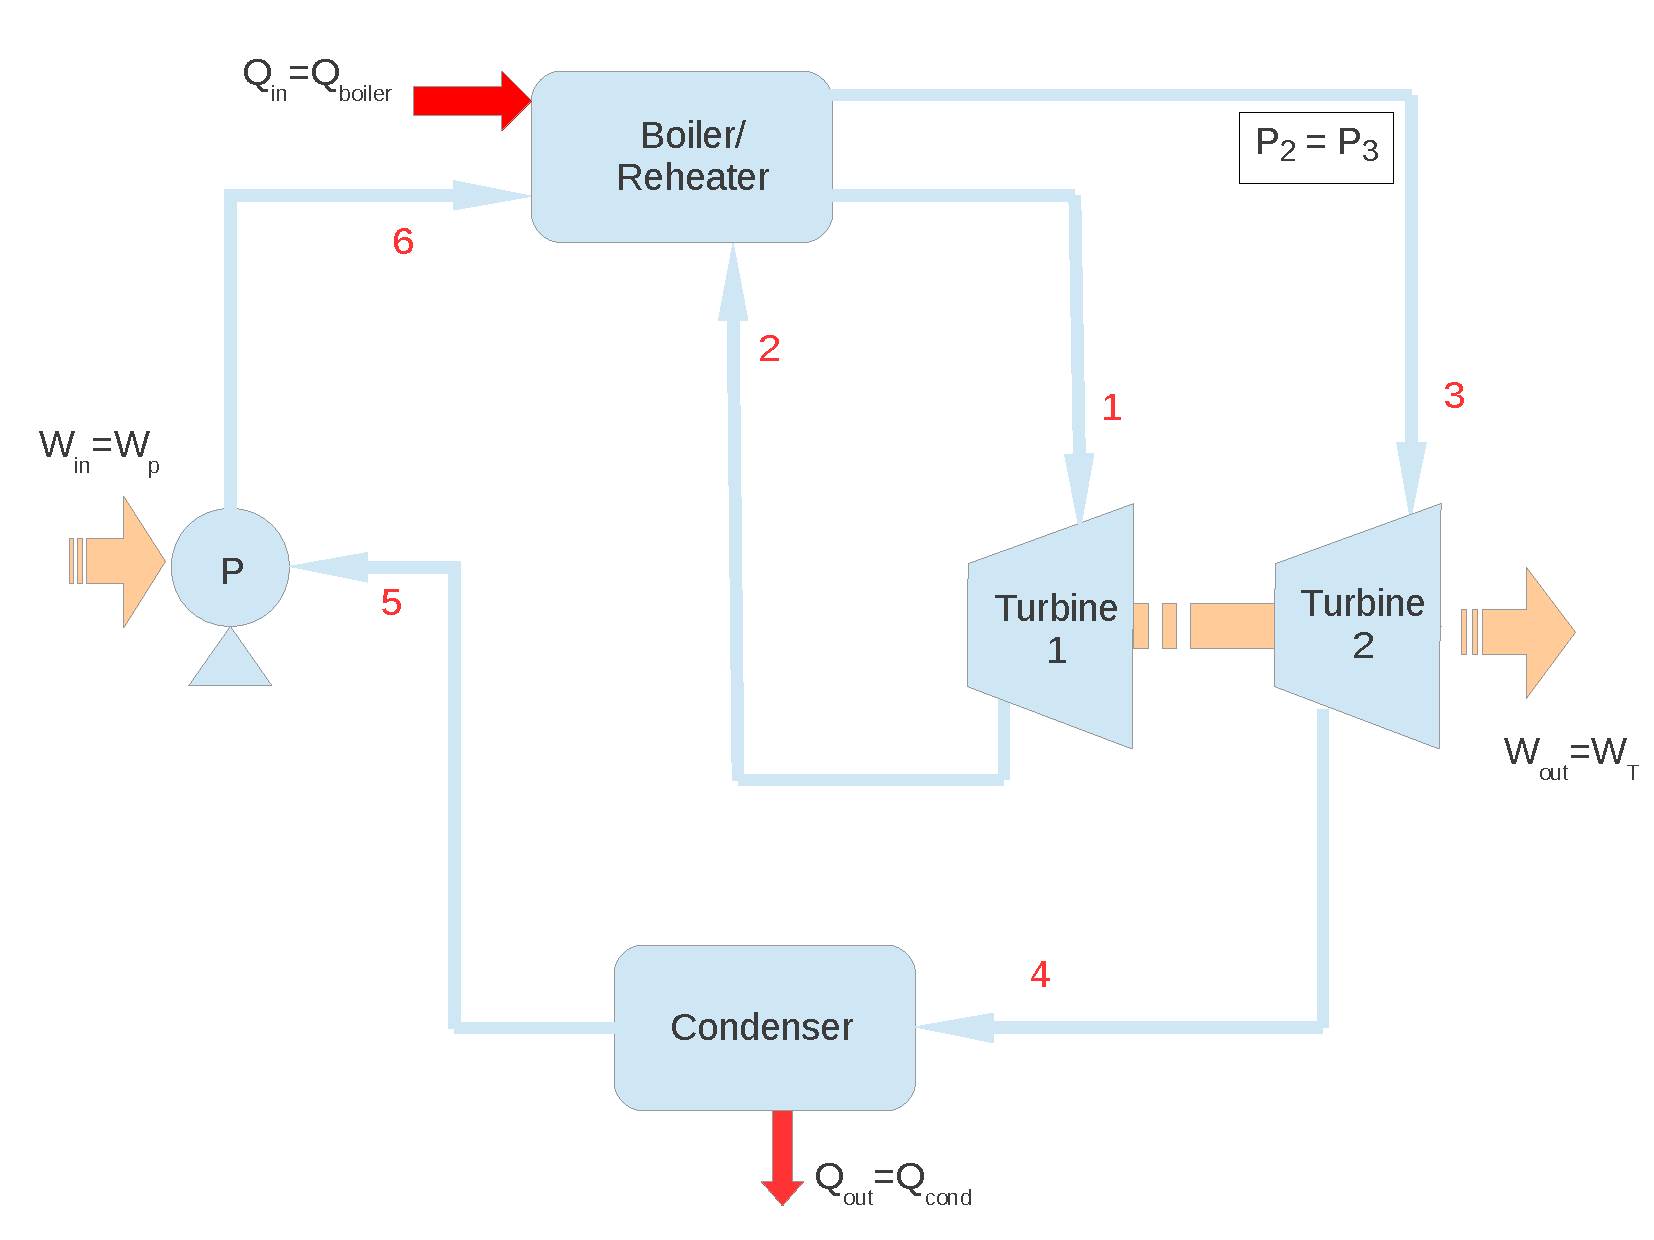
\includegraphics[width=15.cm,clip]{./Pics/Exam_Reheat_Rankine_Cycle}
\caption{ Reheat Rankine cycle with 2 turbines.}
\label{exam_mod01_rankinecycle}
\end{center}
\end{figure}


\begin{enumerate}[(a)]
\item In the Table below, determine {\it (a)-(j)}. {\bf [10 Marks]}\\
%\begin{table}[h]
%\label{exam1_table1}
\begin{center}
\begin{tabular} {||c | c c c c c || }
\hline\hline
{\bf Stage} & {\bf P}    & {\bf T}        & {\bf State}    & {\bf H}             & {\bf S}                  \\
            & {\bf (bar)}& {\bf ($^{o}$C)} &               & {\bf (kJ.kg$^{-1}$)} & {\bf (kJ.(kg.K)$^{-1}$)} \\
\hline\hline
 {\bf 1 }   & 40         & 370            &   superheated  & {\bf (a)}           & {\bf (b)}                 \\
            &            &                &   steam        &                     &                           \\
 {\bf 2 }   &  --        &  --            &     {\bf (c)}  & --                  &   --                      \\
 {\bf 3 }   & 7          & 370            &   superheated  & {\bf (d)}           & {\bf (e)}                 \\
            &            &                &   steam        &                     &                           \\
 {\bf 4 }   & 0.10       & --             &     --         & --                   & --                      \\
 {\bf 5 }   & 0.10       & --             &   {\bf (f)}    & {\bf (g)}           & {\bf (h)}                 \\
 {\bf 6 }   & 40         & --             &   {\bf (i)}    & {\bf (j)}           & --                       \\

\hline\hline
\end{tabular}
\end{center}
%\caption{Thermodynamic table of the reheat Rankine cycle.}
%\end{table}


\item Calculate the thermal efficiency $\left(\eta_{\text{Thermal}}\right)$ of the reheat Rankine cycle with 2 turbines. $\eta_{\text{Thermal}}$ is expressed as, 
\begin{displaymath}
\eta_{\text{Thermal}} = \frc{ \left(H_{1}-H_{2s}\right)\eta_{\text{T1}} + \left(H_{3}-H_{4s}\right)\eta_{\text{T2}} - V_{5}\left(P_{6}-P_{5}\right)\eta_{\text{P}}^{-1}} {\left(H_{1}-H_{6}\right)+\left(H_{3}-H_{2}\right)}
\end{displaymath}
where the subscript {\it s} indicates the ideal state. {\bf [5 Marks]}

\item Sketch the {\it T-S} diagram for this cycle. {\bf [5 Marks]}

\end{enumerate}

\end{question}


\clearpage

%%%
%%% Question 2
%%%
\begin{question} \vspace{-2\baselineskip}
\begin{enumerate}[(a)]
\item In France, 421 billion kWh of electricity were made from nuclear fuels in 2011.  If an equivalent amount had been raised from natural gas, what would have been the carbon footprint? {\bf [8 Marks]}\\
{\it Heat of combustion of methane = 889 kJ.mol$^{-1}$ \\
Atomic weights/gmol$^{-1}$: C: 12 \;\; H: 1}
\item Give an example, in qualitative terms, of how a chemical and nuclear explosion can have equivalent blasts if quantities in the former are much larger than in the latter. {\bf [2 Marks]}
\item Coke, of calorific value is 25 MJ.kg$^{-1}$, is used to make heat at 300 MW. It is desired to reduce the carbon footprint by 10$\%$ by blending the coke with citrus peel of calorific value 7 MJ.kg$^{-1}$ whilst maintaining a heat production rate of 300 MW. At what ratios by weight will coke and citrus peel have to be blended? {\bf [8 Marks]}
\item Explain how in the supply of biomass for fuel use forest sustainability is ensured. {\bf [2 Marks]}
\end{enumerate} 

\end{question}

\clearpage


%%%
%%% Question 3
%%%
\begin{question}\vspace{-2\baselineskip}

\begin{enumerate}[(a)]
%
\item A horizontally mounted turbine is housed between circular inlet and outlet pipes of circumference 1 m and 0.6 m, respectively. Assume gas satisfying the steady flow energy conservation
\begin{displaymath}
\frc{ \dot{Q} -\dot{W}_{s}}{\dot{m}} = \left( h_{2}+ \frc{u_{2}^{2}}{2}\right) - \left(h_{1} + \frc{u_{1}^{2}}{2}\right),
\end{displaymath}
flows through the turbine at a steady rate of 4 kg/s. At the inlet (labelled 1), the fluid has a specific enthalpy $h$ of 70 kJ/kg and a velocity $u$ of 30 m/s, while at the outlet (labelled 2), the fluid has a specific enthalpy of 40 kJ/kg. If the gas does work on the turbine at a rate of 30 kW and transfers heat to the surroundings at a rate of 15 kW, then find the change in gas density between the inlet and the outlet. {\bf [4 Marks]}

%
\item For gas flow along a duct whose length is parameterized by $x$ and has slowly-varying cross-sectional area  $A(x)$, use equations corresponding to mass and energy conservation to show that
\begin{displaymath}
\frc{dV}{V} + \frc{d h}{u^{2}} - \frc{dA}{A}=0,
\end{displaymath}
where the specific volume is denoted $V$, the specific enthalpy $h$, and fluid velocity $u$. {\bf [2 Marks]}
\medskip

\item Define the speed of sound $c$ and the Mach number $M\! a$ in a gas. State equations that are appropriate for calculating these quantities in an isentropic gas and define the variables used. {\bf [4 Marks]}
\medskip

\item For an isentropic process show that changes in specific volume are related to changes in pressure ($p$) through
\begin{displaymath}
dV=-\frc{V^{2}}{c^{2}}dp,
\end{displaymath}
and explain how changes in specific enthalpy are related to changes in pressure. {\bf [3 Marks]}
\medskip

\item Hence, for isentropic flow along a duct, show that
\begin{displaymath}
\frc{1}{A\left(1- M\! a^{2}\right)}\frc{dA}{dx} = \frc{1}{\rho \, M\! a^{2}}\frc{d\rho}{dx},
\end{displaymath}
where the gas density is denoted $\rho$. {\bf [5 Marks]}
\medskip

\item Explain with reasoning how the gas density changes for flow along a supersonic diffuser. {\bf [2 Marks]}
%
\end{enumerate}

\end{question}


\clearpage


%%%
%%% Question 4 (Rajput 14.19)
%%%
\begin{question}A refrigerator operating with Freon-12 as a refrigerant fluid produces a cooling effect of 20 kJ/s (Fig. \ref{exam_refrig1}). The engine operates on a vapour-compression refrigeration cycle with pressure limits of 1.509 bar and 9.607 bar. The vapour leaves the evaporator dry saturated and there is no undercooling.  Assume that the compressor operaters at 300 rpm and has a clearance volume of 3$\%$ of stroke volume.  For the compressor assume that the expansion is described by $PV^{1.13}$ = constant. 
\begin{enumerate}[(a)]
\item Determine the power required by the compressor (in $W$). {\bf [10 Marks]}
\item Calculate the piston displacement of the compressor $\left(\text{in } m^{3}\right)$. {\bf [10 Marks]}
\end{enumerate}

\medskip
Given the saturation table of Freon-12:
\begin{center}
\begin{tabular}{|c c| c c c c c c| }
\hline
$T$             & $P_{s}$  & $V_{g}$  & $H_{f}$  & $H_{g}$   &  $S_{f}$   &  $S_{g}$   & {\it Specific Heat} \\
($^{\text{o}}$C)  & (bar)   & $\left(\text{m}^{3}/\text{kg}\right)$ & (kJ/kg) & (kJ/kg) & (kJ/(kg.K)) &  (kJ/(kg.K)) &   (kJ/(kg.K)) \\
\hline
-20   & 1.509 & 0.1088 & 17.8 & 178.61 & 0.073 & 0.7082 & -- \\
40    & 9.607 & --     & 74.53 & 203.05 & 0.2716 & 0.682 & 0.747 \\
\hline
\end{tabular}
\end{center}
where $T$ and $P$ are temperature and saturated pressure, respectively; $V$, $H$ and $S$ are the specific volume, enthalpy and entropy. Subscripts $f$ and $g$ represents fluid and gas/vapour phases. Swept volume rate $\left(\dot{V}_{\text{swept}}\right)$ and volumetric efficiency $\left(\eta_{\text{vol}}\right)$ are expressed as,
\begin{eqnarray}
&& \dot{V}_{\text{swept}} = \frc{\dot{V}_{R}}{\eta_{\text{vol}}} \nonumber \\
&& \eta_{\text{vol}} = 1 + \mathcal{C} - \mathcal{C}\left(\frc{P_{d}}{P_{s}}\right)^{1/n} \nonumber  
\end{eqnarray}
where $\dot{V}_{R}$ is the volumetric flow rate of the refrigerant at intake conditions, $\mathcal{C}$ is the clearance ratio, $P_{d}$ and $P_{s}$ are the discharge and suction pressures, respectively. $n$ is the polytropic index.


\begin{figure}[h]
\begin{center}
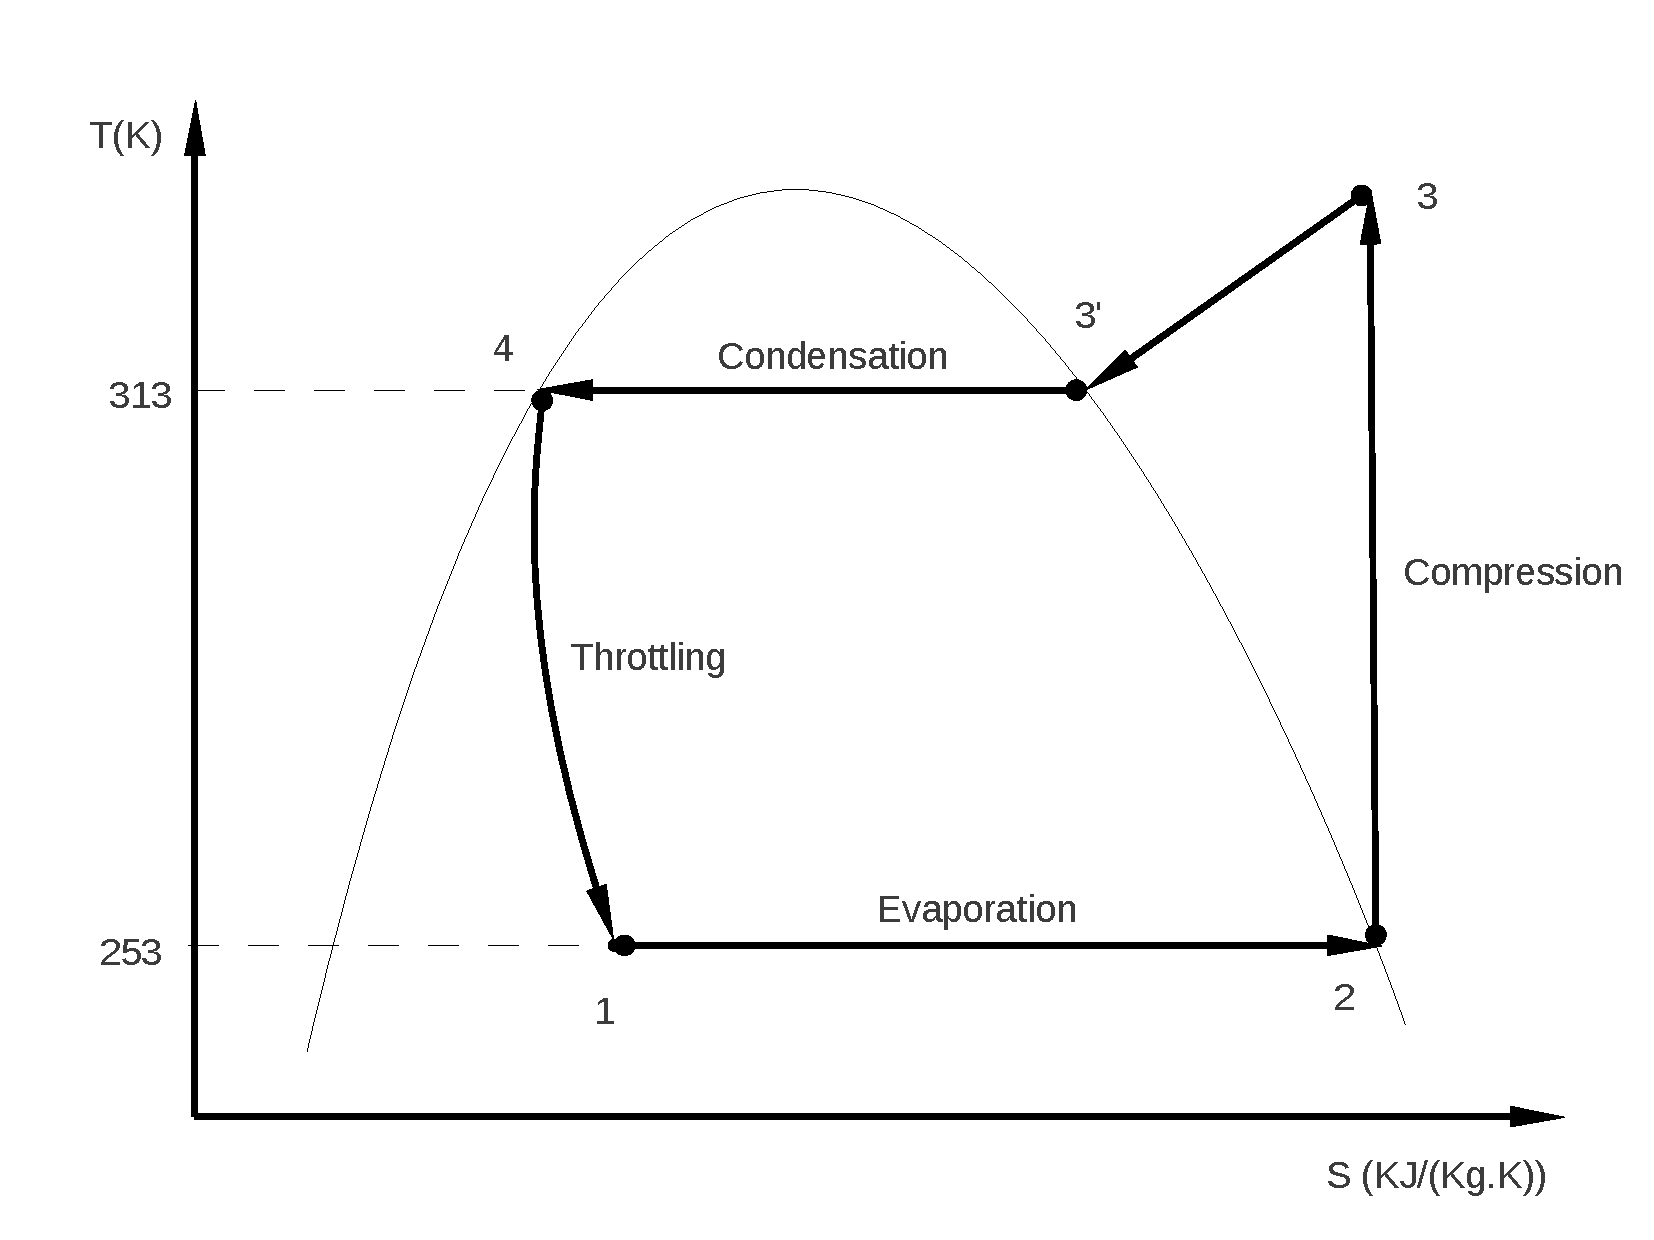
\includegraphics[width=10.cm,clip]{./Pics/Exam_Refrigeration1}
\caption{ Refrigeration cycle, $Ts$ diagram  -- Question 4}
\label{exam_refrig1}
\end{center}
\end{figure}


\end{question}

\clearpage


%%%
%%% Question 5
%%%
\begin{question}\vspace{-2\baselineskip}

\begin{enumerate}[(a)]
\item Define the specific humidity $\omega$. Assuming both dry air and water vapour behave like ideal gases with specific gas constants $R_{a}=0.2871$ kJ/(kg.K) and $R_{v}=0.4615$ kJ/(kg.K), respectively, show that
\begin{displaymath}
\omega = \frc{0.622 p_{v}}{p-p_{v}}
\end{displaymath}
where $p$ is the absolute pressure and $p_{v}$ is the partial pressure of water vapour. {\bf [4 Marks]}
\medskip

\item If the saturation pressure of water is denoted $p_{g}$, and relative humidity $\varphi$, then show that {\bf [2 Marks]}
\begin{displaymath}
\omega = \frc{0.622 \varphi p_{g}}{p-\varphi p_{g}}
\end{displaymath}
\medskip

\item An air-conditioning system takes in outdoor air at 12$^{\text{o}}$C and 25 percent relative humidity at a steady rate of 40 m$^{3}$/min and then conditions it to 24$^{\text{o}}$C and 55 percent relative humidity. This heating and humidification takes place in two distinct steady processes. Firstly the outdoor air is heated to 20$^{\text{o}}$C in a heating section, and secondly the air is humidified by the injection of hot steam in a humidifying section. Assuming both stages take place at a constant pressure of 100 kPa, determine:
\begin{enumerate}[(i)]
\item the partial pressures of water vapour and dry air, and the specific humidity at the inlet; {\bf [3 Marks]}  
\item the rate heat is supplied in the heating section;  {\bf [6 Marks]}
\item the mass flow rate of the steam required in the humidifying section. {\bf [5 Marks]}
\end{enumerate}
\medskip
\end{enumerate}
You may assume that the specific heat of dry air is independent of temperature and has the value $C_{p}=1.005$ kJ/(kg.K). The saturation pressure of water is 1.4028 kPa at 12$^{\text{o}}$C, and 2.9858 kPa at 24$^{\text{o}}$C. The enthalpy of saturated water vapour is 2523 kJ/kg at 12$^{\text{o}}$C, and 2537 kJ/kg at 20$^{\text{o}}$C.

\end{question}



\vfill

\paperend
\end{document}
